\subsection{Decisiones cerradas y alcance de esta actualización}

La actualización del 18 de octubre de 2026 conserva ocho candidatas: 1HM, 2HM, seis materiales agregados de 6V, energía, gas e internet de 8V, 10V y actividad ponderada 5PM. Basuras queda fuera de ese conjunto y se examina exclusivamente como sensibilidad exploratoria. Se mantiene 17PM reservada, 1PM y 1V como contexto, y 6PM excluida. Las quince privaciones del IPM permanecen fuera de la matriz. El equipo aprobó conservar las candidatas pese a su proximidad temática con el IPM, hacer explícita esa proximidad y comparar posteriormente soluciones que retiren las más cercanas. Esta corrida calcula descriptivos y sensibilidad de fórmulas y correlaciones; no ejecuta PCA, KMO, Bartlett ni construcción del IVS.

\subsection{Justificación específica y límites de las aproximaciones}

El marco de activos y oportunidades fundamenta una lectura multidimensional de restricciones y recursos \citep{kaztman1999activos,pizarro2001vulnerabilidad}. El antecedente colombiano ICVU incorpora cuidado, condiciones habitacionales y acceso a bienes; utiliza hogares y otro método, por lo que respalda la pertinencia de esos dominios, sin validar nuestras fórmulas municipales \citep{dnp2023icvu}. Para cada candidata se conserva la definición y el denominador de la \cref{tab:formulas_candidatas}, con las siguientes precisiones:

\begin{description}[leftmargin=1.27cm,style=nextline]
\item[1HM y 2HM: composición del hogar y cuidado potencial.] Son proporciones de hogares con presencia de los grupos de edad elegidos. Su dirección positiva es una hipótesis operacional del equipo. El antecedente sobre cuidado respalda explorar el dominio, pero la edad no determina necesidad de ayuda: no se observan horas de cuidado, autonomía, apoyos ni dependencia económica. Los hogares pueden pertenecer a ambas categorías; no son partes de una distribución exhaustiva \citep{dnp2023icvu,dane2021cnpv}.
\item[6V: composición material de las paredes.] Se mantiene la agregación de seis materiales aprobada. La calidad de vivienda es pertinente para estudiar condiciones de vida, pero el material aislado no informa estado constructivo, mantenimiento, riesgo local ni adecuación cultural. En particular, incluir guadua y tapia/bahareque/adobe no implica que toda construcción con esos materiales sea insegura. El nombre operativo \texttt{paredes\_precarias\_6V} designa la agrupación del proyecto, no una clasificación oficial de déficit. Se publican las seis proporciones para examinar sus contribuciones \citep{dane2021cnpv,dnp2023icvu}.
\item[Energía, gas e internet (8V): acceso diferenciado.] Las tres proporciones describen carencia declarada del servicio correspondiente entre viviendas ocupadas con personas presentes. La falta de gas por red puede relacionarse con oferta territorial y combustibles alternativos; no mide por sí sola falta de energía para cocinar. La ausencia de internet no informa calidad, uso ni habilidades digitales. Se conservan como aproximaciones diferenciadas y se examinan denominadores y correlaciones, sin atribuirles equivalencia sustantiva \citep{dane2021cnpv}.
\item[10V: clasificación socioeconómica asociada al inmueble.] El DANE fundamenta la estratificación en características del inmueble para servicios públicos. Esa finalidad respalda un uso contextual; no demuestra que todas las personas sin estrato sean vulnerables. El corte 1--2, la inclusión de \enquote{No tiene estrato} y la dirección positiva son decisiones del equipo. La proporción condiciona en estratos 1--6 más \enquote{No tiene estrato}; no mide prevalencia entre toda la población. Las categorías sin servicio de energía y no respuesta permanecen separadas. La Ley 142 no se utiliza como prueba de validez de este numerador \citep{dane_estratificacion}.
\item[5PM: puntuación experimental de actividad de población 10+.] Las categorías proceden de la actividad de la semana anterior. La suma ponderada representa una decisión operacional de relevancia relativa, sin identificar desempleo oficial ni dependencia de hogares. El peso 2:1 es normativo; la literatura diferencia este tipo de pesos de los empíricos, pero no prescribe el valor dos. Los escenarios 1:1 y 3:1 hacen visible el efecto de esa elección \citep{dane_5pm,decancq2013weights}.
\end{description}

Estas razones justifican estudiar las candidatas con límites explícitos. No constituyen una demostración de que la combinación mida toda la vulnerabilidad. La selección contiene decisiones normativas que deben permanecer visibles aun cuando los cálculos sean exactos \citep{oecd2008composite,alkire2011multidimensional}.

\subsection{Proximidad con el IPM: contraste convergente parcial}

El IPM censal caracteriza privaciones del hogar con reglas propias. En paredes, sus criterios cambian entre urbano y rural; en dependencia utiliza personas por ocupado. Por ello, compartir dominio no implica usar la misma medida \citep{dane2020ipmcensal}. Además de la proximidad conceptual, ambas construcciones comparten fuente censal: una asociación posterior no será evidencia de validación independiente.

\begin{table}[htbp]
\centering\small
\caption{Proximidad conceptual de candidatas con privaciones del IPM}\label{tab:solapamiento_actual}
\begin{tabularx}{\textwidth}{@{}lXX@{}}
\toprule
Candidata & Privación o dominio cercano & Distinción y escenario acordado \\
\midrule
1HM / 2HM & Cuidado de primera infancia; dependencia & Presencia etaria no equivale a personas por ocupado. Comparar posteriormente sin ambas. \\
5PM & Dependencia; trabajo informal e infantil & Población 10+, categorías y pesos diferentes; vínculo indirecto. \\
6V & Material de paredes exteriores & Cercanía directa parcial; agrupación y unidad distintas. Comparar sin 6V y con sus componentes. \\
Energía / gas & Servicios y condiciones de vida & No hay privación idéntica de esos servicios en las quince publicadas. \\
Internet & Educación y oportunidades & Asociación temática indirecta, sin privación equivalente. \\
10V & Vivienda y servicios & El IPM no incluye estrato; uso administrativo como aproximación. \\
17PM & Bajo logro; analfabetismo; trayectoria escolar & Edad 5+ y medida distintas; se reserva para exploración posterior. \\
\bottomrule
\end{tabularx}
\end{table}

Agua y alcantarillado se conservan fuera de los ocho por la decisión acordada de reducir proximidad temática. Ese criterio no se interpreta como ausencia total de solapamiento en las candidatas retenidas. La tabla documenta una evaluación conceptual; no es un test estadístico ni usa correlaciones altas como regla de selección.

\subsection{Universo descriptivo y estimandos}

Se verificaron los veinte códigos ANM en la capa histórica \emph{Serv\_DeptosMpiosANM\_2018}, consultada el 18 de octubre; incluye 94343 y 94663. La transcripción reproducible se conserva en \path{docs/metodologia/anm_divipola_2018_verificadas_20261018.csv}. El resto del conjunto censal contiene 1.101 municipios/distritos y la unidad insular 88001. Esta presentación sigue la distinción territorial del CNPV \citep{dane2018divipola,dane2021cnpv}.

La tabla principal describe el \textbf{ámbito municipal e insular de 1.102 unidades}, con las ANM fuera. Se guardan también los descriptivos para 1.101 municipios/distritos, las veinte ANM y los 1.122 códigos completos. Incluir San Andrés en esta tabla descriptiva no cierra su participación en el futuro PCA; la decisión analítica final debe explicitar ese caso.

Para el indicador $x_i=N_i/D_i$, cada unidad territorial tiene el mismo peso en la media y la desviación descriptiva:
\begin{equation}
\bar{x}=\frac{1}{m}\sum_{i=1}^{m}x_i,\qquad
\sigma_x=\sqrt{\frac{1}{m}\sum_{i=1}^{m}(x_i-\bar{x})^2},\qquad
p_A=\frac{\sum_iN_i}{\sum_iD_i}=\sum_i\frac{D_i}{\sum_k D_k}x_i.
\end{equation}
La tabla emplea DE con divisor $m$, porque describe el universo observado; el CSV añade la DE convencional con divisor $m-1$ para comparación. Los cuartiles usan el método 7 de \texttt{quantile} en R \citep{r_core_team}. La razón $p_A$ pondera por el denominador y corresponde a otro estimando. No se presentan intervalos de confianza muestrales ni pruebas de medias entre municipios: las estadísticas describen cobertura censada, con posibles errores de cobertura y medición, no una muestra probabilística de municipios.

\begin{table}[htbp]
\centering\small
\caption{Distribución territorial de cuatro indicadores aprobados, en porcentaje}\label{tab:descriptivos_cuatro_actual}
\begin{adjustbox}{max width=\textwidth}
\begin{tabular}{@{}lrrrrrrrr@{}}
\toprule
Indicador & $n$ & Media & DE & Mediana & Q1 & Q3 & Mín. & Máx. \\
\midrule
1HM & 1102 & 45,60 & 8,97 & 44,78 & 38,87 & 52,16 & 22,49 & 79,18 \\
6V & 1102 & 31,03 & 22,03 & 27,50 & 12,72 & 45,43 & 0,11 & 97,89 \\
Energia & 1102 & 7,63 & 12,41 & 3,19 & 1,47 & 7,48 & 0,09 & 95,87 \\
10V & 1102 & 93,85 & 11,14 & 98,76 & 93,00 & 99,70 & 23,19 & 100,00 \\
\bottomrule
\end{tabular}

\end{adjustbox}
\par\footnotesize Fuente: \path{descriptivos_cuatro_informe.csv}, generado por \path{R/06_descriptivos_sensibilidades_ivs.R}. Ámbito: municipios/distritos y San Andrés; excluye ANM. DE poblacional.
\end{table}

La distancia entre media y mediana de energía y paredes muestra heterogeneidad territorial; una media simple municipal no representa la proporción de viviendas del país. En 10V la mediana cercana al límite superior obliga a examinar concentración y capacidad de discriminación; no significa que esa proporción de personas sea pobre según una definición oficial. La agrupación de paredes y la población elegible de estrato deben conservarse al interpretar estas distribuciones.

\begin{table}[htbp]
\centering\small
\caption{Razones de sumas para el mismo ámbito municipal e insular}\label{tab:razones_sumas_actual}
\begin{adjustbox}{max width=\textwidth}
\begin{tabular}{@{}lrrr@{}}
\toprule
Indicador & Numerador agregado & Denominador agregado & Razón (\%) \\
\midrule
1HM & 6212256 & 14236949 & 43,63 \\
6V & 1734392 & 13474496 & 12,87 \\
Energia & 492244 & 13474496 & 3,65 \\
10V & 30704989 & 42013803 & 73,08 \\
\bottomrule
\end{tabular}

\end{adjustbox}
\par\footnotesize Fuente: \path{descriptivos_cuatro_informe.csv}. Son agregaciones de conteos publicados del ámbito descrito, no tasas nacionales oficiales ni estimaciones corregidas por omisión censal.
\end{table}

\begin{figure}[htbp]
\centering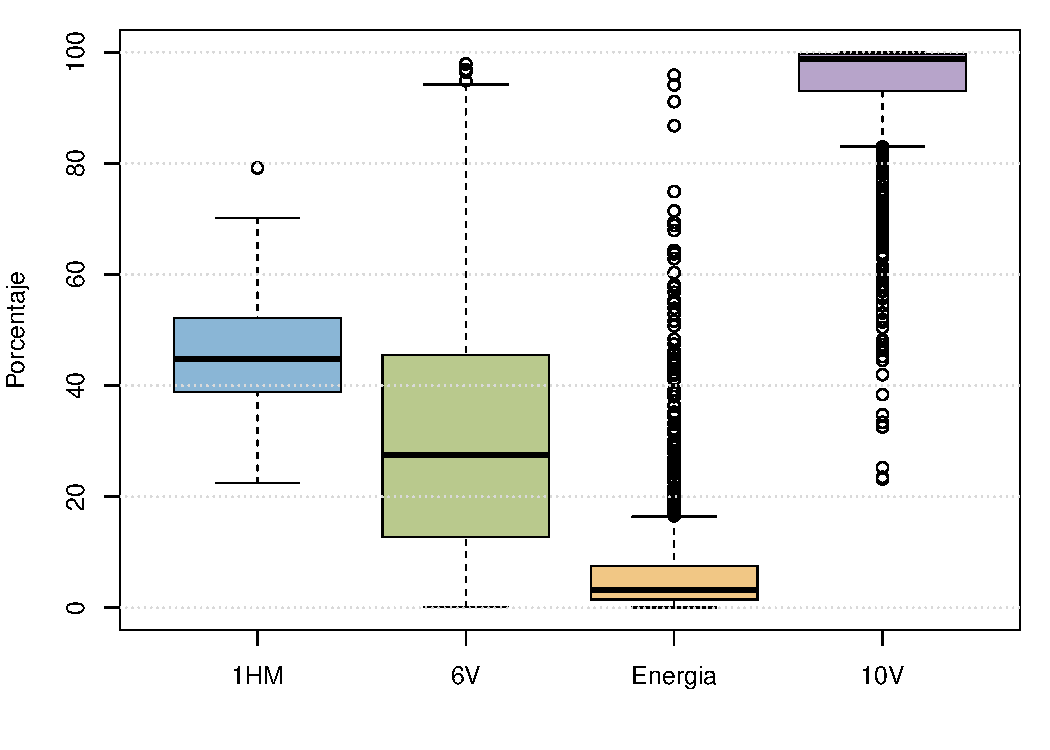
\includegraphics[width=.9\textwidth]{../../resultados/descriptivos_sensibilidades_20261018/figuras/distribuciones_cuatro.pdf}
\caption{Distribuciones de cuatro candidatas en el ámbito municipal e insular. Las cajas muestran mediana e intervalo intercuartílico; los bigotes se extienden hasta los datos dentro de 1,5 veces ese intervalo. Los puntos exteriores se conservan. Fuente: matriz recalculada de ocho indicadores.}
\end{figure}

\subsection{Sensibilidad de fórmulas y no respuesta}

La comparación utiliza las mismas unidades y define $\Delta_i=x_i^{(a)}-x_i^{(0)}$. Se reportan media de $|\Delta_i|$, máximo, número de casos con $|\Delta_i|\geq0,02$ y correlación entre rangos con empates promediados, $\rho_s=\operatorname{cor}(\operatorname{rango}(x^{(0)}),\operatorname{rango}(x^{(a)}))$. El umbral de dos puntos porcentuales es descriptivo, no un nivel de significancia. La exploración de supuestos de normalización y ponderación sigue las recomendaciones de transparencia y sensibilidad para indicadores compuestos \citep{oecd2008composite,decancq2013weights}.

En 5PM, con $U$ trabajo no remunerado, $B$ búsqueda, $C$ incapacidad y $V=T-NR$, la alternativa de peso $w\in\{1,2,3\}$ es
\begin{equation}
L_w=\frac{U+B+wC}{wV}=\frac{C}{V}+\frac{U+B}{wV}.
\end{equation}
La normalización por el peso máximo conserva el rango [0,1]: al aumentar $w$ mantiene el aporte normalizado de incapacidad y reduce el de las otras dos categorías. Por ello, los deltas reflejan conjuntamente ponderación relativa y normalización; no son cambios observados de actividad de la población.

Para gas e internet, si $N$ es carencia observada, $T$ total y $R$ no respuesta, se conservan:
\begin{equation}
p_{\text{válido}}=\frac{N}{T-R},\qquad
p_{\mathrm{inferior}}=\frac{N}{T},\qquad
p_{\mathrm{superior}}=\frac{N+R}{T}.
\end{equation}
Las cotas asignan a toda NR respectivamente ausencia o presencia de carencia. Son escenarios extremos de asignación, no intervalos de confianza. El denominador válido describe las respuestas observadas; extenderlo a todas las viviendas requeriría hipótesis sobre el mecanismo de NR que aquí no se asumen. Para 5PM, el escenario de cota asigna puntuación máxima a NR y normaliza por $2T$. Para 10V, incluir personas sin energía en el denominador cambia también la población objetivo: no es solo un ajuste de NR.

\begin{table}[htbp]
\centering\small
\caption{Sensibilidad de fórmulas en las 1.102 unidades municipales e insulares}\label{tab:sensibilidad_actual}
\begin{adjustbox}{max width=\textwidth}
\begin{tabular}{@{}lrrrr@{}}
\toprule
Alternativa & $\rho_s$ & $|\Delta|$ medio (pp) & $|\Delta|$ máx. (pp) & $\geq2$ pp \\
\midrule
5PM: peso 1:1 & 0,948 & 2,75 & 21,43 & 698 \\
5PM: peso 3:1 & 0,975 & 0,92 & 7,14 & 44 \\
5PM: total & 0,999 & 0,09 & 0,84 & 0 \\
5PM: cota NR & 0,858 & 1,79 & 18,26 & 216 \\
Gas: total & 0,994 & 0,54 & 12,46 & 52 \\
Internet: total & 0,968 & 0,75 & 14,01 & 69 \\
10V: total & 0,446 & 7,44 & 97,62 & 691 \\
17PM: Normal incompleta & 0,998 & 0,28 & 4,79 & 12 \\
17PM: base válida & 0,968 & 1,11 & 21,41 & 86 \\
\bottomrule
\end{tabular}

\end{adjustbox}
\par\footnotesize Fuente: \path{sensibilidades_formulas_por_ambito.csv}. Cada alternativa se compara con su fórmula principal. 17PM permanece fuera de las ocho candidatas; sus filas son exploratorias.
\end{table}

Al separar ANM cambia el conjunto de comparación respecto de la tabla histórica de 1.122 códigos: por ejemplo, los conteos del peso 5PM y del denominador 10V no deben trasladarse de una tabla a otra. El cambio a peso 1:1 tiene mayor efecto que el cambio a 3:1 bajo la normalización elegida; esa asimetría no demuestra que el peso dos sea óptimo. En 10V, la elevada sensibilidad revela que la interpretación condicionada al denominador es esencial. Las fórmulas aprobadas se conservan, con esas cautelas.

\begin{figure}[htbp]
\centering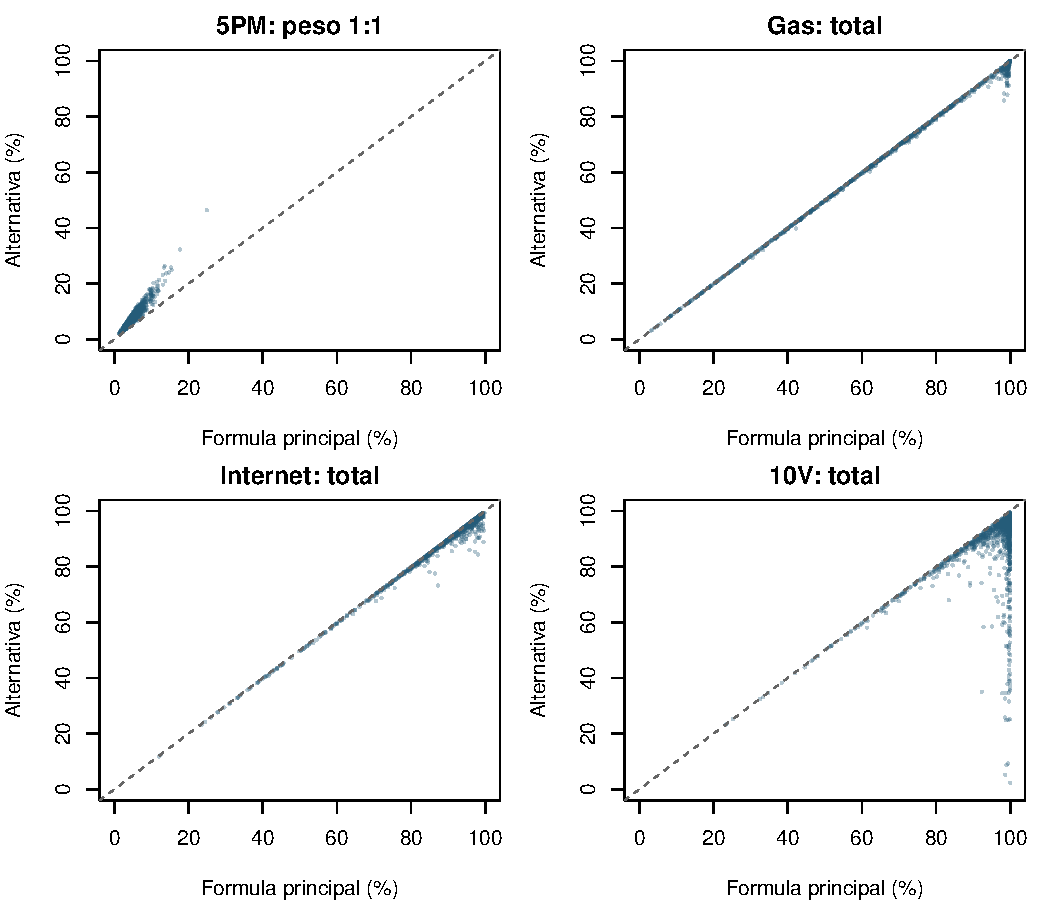
\includegraphics[width=.95\textwidth]{../../resultados/descriptivos_sensibilidades_20261018/figuras/sensibilidad_denominadores.pdf}
\caption{Fórmula principal frente a alternativas de peso y denominador. La diagonal indica igualdad; cada punto corresponde a una unidad municipal o insular. Fuente: sensibilidades por código.}
\end{figure}

\subsection{Sensibilidad de correlaciones, sin componentes principales}

Para evaluar efectos sobre las asociaciones se calculan matrices de Pearson y Spearman por escenario. Sobre los pares comunes $\mathcal{P}$ se resumen
\begin{equation}
\Delta_r^{\max}=\max_{(j,k)\in\mathcal P}|r_{jk}^{(a)}-r_{jk}^{(0)}|,\qquad
\mathrm{RDCM}_r=\sqrt{\frac{1}{|\mathcal P|}\sum_{(j,k)\in\mathcal P}(r_{jk}^{(a)}-r_{jk}^{(0)})^2}.
\end{equation}
Estas medidas describen cambios de asociación; no son contrastes de hipótesis. Spearman permite comprobar si las relaciones monotónicas difieren de las lineales; ninguna de las dos elimina por sí sola el efecto de agregación territorial ni garantiza una estructura dimensional adecuada \citep{jolliffe2002principal}.

En el escenario principal, Pearson entre 1HM y 2HM es $-0,721$, mientras que entre internet y 10V es $0,833$ (\path{correlaciones_escenarios.csv}). La primera relación indica estructuras territoriales de hogares contrapuestas, aunque ambas candidatas tengan dirección conceptual positiva; no implica corregir signos automáticamente. La segunda motiva evaluar redundancia estadística, aunque los conceptos difieran. Ninguna anticipa por sí sola cargas o dimensiones del PCA pendiente.

\begin{table}[htbp]
\centering\small
\caption{Cambios de correlación de Pearson bajo alternativas, sobre 28 pares comunes}\label{tab:corr_sensibilidad_actual}
\begin{adjustbox}{max width=\textwidth}
\begin{tabular}{@{}lrr@{}}
\toprule
Alternativa & Máximo $|\Delta r|$ & Raíz de diferencia cuadrática media \\
\midrule
5PM: peso 1:1 & 0,163 & 0,048 \\
5PM: peso 3:1 & 0,111 & 0,032 \\
5PM: total & 0,015 & 0,004 \\
5PM: cota NR & 0,335 & 0,090 \\
Gas: total & 0,015 & 0,004 \\
Internet: total & 0,047 & 0,013 \\
10V: total & 0,909 & 0,259 \\
Gas e internet: total & 0,047 & 0,013 \\
\bottomrule
\end{tabular}

\end{adjustbox}
\par\footnotesize Fuente: \path{sensibilidad_correlaciones.csv}. Las matrices completas y las versiones Spearman se conservan en \path{correlaciones_escenarios.csv}.
\end{table}

La alternativa de 10V modifica las asociaciones mucho más que las variantes de gas e internet. Eso motiva mantener visible la definición condicional y exigir sensibilidad dimensional en la siguiente fase. También se guardan matrices con basuras, 17PM, paredes desagregadas y retiro de candidatas próximas al IPM. Retirar o añadir columnas deja iguales las correlaciones entre las variables conservadas: un delta cero en esos pares es una identidad del cálculo, no evidencia de estabilidad de componentes o rankings. Evaluar esa estabilidad requiere el PCA, expresamente diferido.

\subsection{Valores extremos, integridad y cuestiones pendientes}

La matriz de ocho candidatas en el ámbito municipal e insular registra 43 códigos con 47 celdas cuyo $|z|>4$, usando la desviación convencional para mantener la regla histórica. El cotejo independiente con los valores cacheados del Excel identifica hoja, fila, numerador y denominador para cada celda: ninguna supera una diferencia de $10^{-12}$. Se preservan todas las observaciones. El detalle está en \path{cotejo_extremos_excel.csv}; confirmar la transcripción no valida el fenómeno en campo. Los 32 casos de la matriz histórica de siete variables pertenecen a otra especificación y no se sustituyen retrospectivamente por esta lista.

Los hash de los insumos antes y después coinciden, según \path{integridad_insumos.csv}; el cotejo del libro añade SHA-256 en \path{integridad_excel_cotejo.csv}. La salida \path{resumen_ejecucion.csv} registra ocho candidatas sin NA, cero diferencias de fórmula y PCA no ejecutado. La revisión bibliográfica corrigió el DOI de Kaiser y la autoría del artículo de Monsalvo Herrera y Jiménez a partir de las páginas editoriales. No se atribuye respaldo empírico al peso 2:1 ni a \enquote{No tiene estrato} que las fuentes no proporcionan.

Quedan pendientes la decisión final sobre San Andrés en el PCA municipal, los enlaces territoriales para SECOP, los diagnósticos de adecuación de la matriz definitiva, la retención e interpretación de componentes, la estabilidad de sus cargas y puntajes, y la regla de construcción del IVS. El trabajo actual cierra fórmulas, clasificación histórica ANM y evidencia descriptiva; el alcance de la justificación sigue siendo explícitamente parcial para las decisiones normativas. El CSV histórico conserva una instrucción residual en el campo de verificación de 6PM sobre desocupación: no se aplica, pues el acuerdo vigente excluye ese cuadro. La nota de actualización registra esa inconsistencia sin alterar el archivo histórico.
